%
% einleitung.tex -- Beispiel-File für die Einleitung
%
% (c) 2020 Prof Dr Andreas Müller, Hochschule Rapperswil
%
% !TEX root = ../../buch.tex
% !TEX encoding = UTF-8
%
\section{Ein Moderner Beweis}
\label{basel:section:modernerbeweis}

Wir arbeiten mit der Funktion $x \to x^2$ auf $[-\pi, \pi)$.

\begin{figure}
\centering
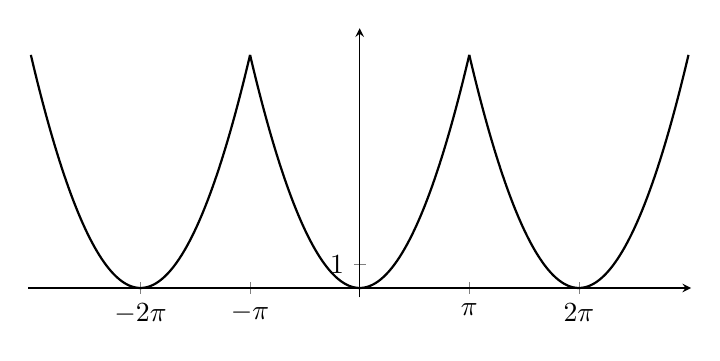
\begin{tikzpicture}
\begin{axis}[
    width=10cm, height=5cm,
    xmin=-9.5, xmax=9.5,
    ymin=-0.4, ymax=11,
    xtick={-6.2832,-3.1416,0,3.1416,6.2832},
    xticklabels={$-2\pi$,$-\pi$,$0$,$\pi$,$2\pi$},
    ytick={1},
    axis lines=center,
    samples=300,
    clip=false,
]
\addplot[thick, domain=-3.1416:3.1416]         {x^2};
\addplot[thick, domain=-9.4248:-3.1416]        {(x+6.2832)^2};
\addplot[thick, domain=3.1416:9.4248]          {(x-6.2832)^2};
\end{axis}
\end{tikzpicture}
\caption{Die periodisch fortgesetzte Funktion $f(x)=x^2$ auf $[-\pi,\pi)$.
\label{basel:figure:f}}
\end{figure}

Wir führen eine Fourier-Analyse dieser Funktion durch.
Die Darstellung von Funktionen als unendliche Summen von trigonometrischen Funktionen
ist etwas, worüber Euler auch schon nachgedacht hat,
aber er kam nie so weit, dass man hier von einer Theorie sprechen konnte.

Das nullte Fourierpolynom von unserer Funktion ist nicht besonders,
denn es ist nur eine konstante Funktion.

\begin{figure}
\centering
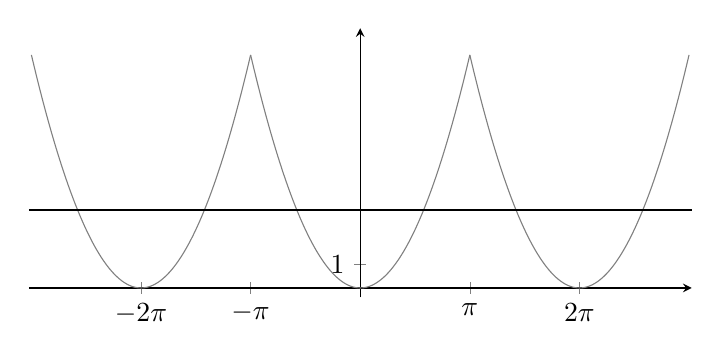
\begin{tikzpicture}
\begin{axis}[
    width=10cm, height=5cm,
    xmin=-9.5, xmax=9.5,
    ymin=-0.4, ymax=11,
    xtick={-6.2832,-3.1416,0,3.1416,6.2832},
    xticklabels={$-2\pi$,$-\pi$,$0$,$\pi$,$2\pi$},
    ytick={1},
    axis lines=center,
    samples=300,
    clip=false,
]
\addplot[thin, gray, domain=-3.1416:3.1416]    {x^2};
\addplot[thin, gray, domain=-9.4248:-3.1416]   {(x+6.2832)^2};
\addplot[thin, gray, domain=3.1416:9.4248]     {(x-6.2832)^2};
\addplot[thick, domain=-9.5:9.5]               {9.8696/3};
\end{axis}
\end{tikzpicture}
\caption{Nulltes Fourierpolynom: konstante Approximation $\frac{\pi^2}{3} \approx 3.29$.
\label{basel:figure:fourier0}}
\end{figure}

Erstes Fourierpolynom:

\begin{figure}
\centering
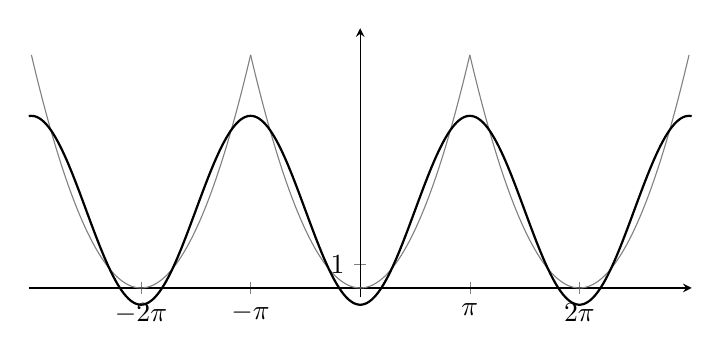
\begin{tikzpicture}
\begin{axis}[
    width=10cm, height=5cm,
    xmin=-9.5, xmax=9.5,
    ymin=-0.4, ymax=11,
    xtick={-6.2832,-3.1416,0,3.1416,6.2832},
    xticklabels={$-2\pi$,$-\pi$,$0$,$\pi$,$2\pi$},
    ytick={1},
    axis lines=center,
    samples=300,
    clip=false,
]
\addplot[thin, gray, domain=-3.1416:3.1416]    {x^2};
\addplot[thin, gray, domain=-9.4248:-3.1416]   {(x+6.2832)^2};
\addplot[thin, gray, domain=3.1416:9.4248]     {(x-6.2832)^2};
\addplot[thick, domain=-9.5:9.5]
    {9.8696/3 - 4*cos(deg(x))};
\end{axis}
\end{tikzpicture}
\caption{Erstes Fourierpolynom.
\label{basel:figure:fourier1}}
\end{figure}

Zweites Fourierpolynom:

\begin{figure}
\centering
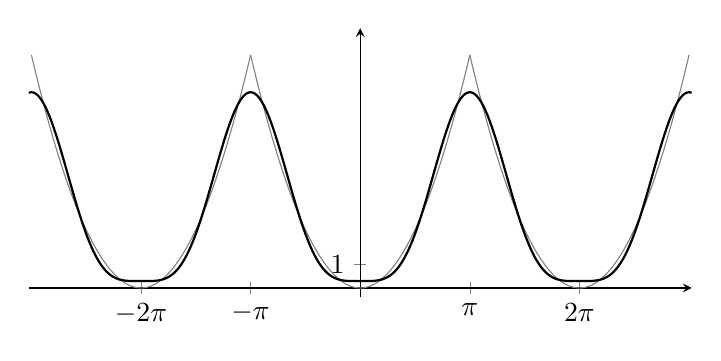
\begin{tikzpicture}
\begin{axis}[
    width=10cm, height=5cm,
    xmin=-9.5, xmax=9.5,
    ymin=-0.4, ymax=11,
    xtick={-6.2832,-3.1416,0,3.1416,6.2832},
    xticklabels={$-2\pi$,$-\pi$,$0$,$\pi$,$2\pi$},
    ytick={1},
    axis lines=center,
    samples=300,
    clip=false,
]
\addplot[thin, gray, domain=-3.1416:3.1416]    {x^2};
\addplot[thin, gray, domain=-9.4248:-3.1416]   {(x+6.2832)^2};
\addplot[thin, gray, domain=3.1416:9.4248]     {(x-6.2832)^2};
\addplot[thick, domain=-9.5:9.5]
    {9.8696/3 - 4*cos(deg(x)) + cos(deg(2*x))};
\end{axis}
\end{tikzpicture}
\caption{Zweites Fourierpolynom.
\label{basel:figure:fourier2}}
\end{figure}

Drittes Fourierpolynom:

\begin{figure}
\centering
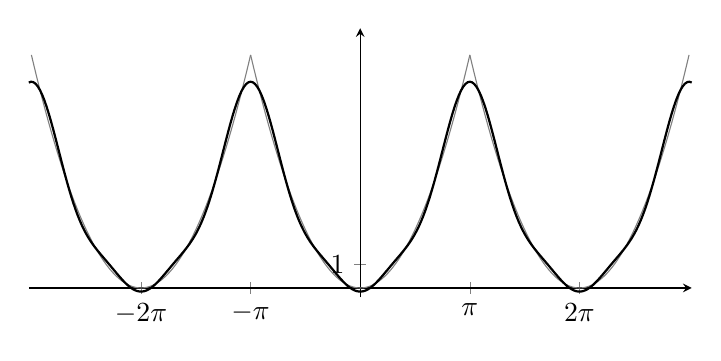
\begin{tikzpicture}
\begin{axis}[
    width=10cm, height=5cm,
    xmin=-9.5, xmax=9.5,
    ymin=-0.4, ymax=11,
    xtick={-6.2832,-3.1416,0,3.1416,6.2832},
    xticklabels={$-2\pi$,$-\pi$,$0$,$\pi$,$2\pi$},
    ytick={1},
    axis lines=center,
    samples=300,
    clip=false,
]
\addplot[thin, gray, domain=-3.1416:3.1416]    {x^2};
\addplot[thin, gray, domain=-9.4248:-3.1416]   {(x+6.2832)^2};
\addplot[thin, gray, domain=3.1416:9.4248]     {(x-6.2832)^2};
\addplot[thick, domain=-9.5:9.5]
    {9.8696/3 - 4*cos(deg(x)) + cos(deg(2*x)) - (4/9)*cos(deg(3*x))};
\end{axis}
\end{tikzpicture}
\caption{Drittes Fourierpolynom.
\label{basel:figure:fourier3}}
\end{figure}

Anhand der Beobachtung dieser Polynome wird die Näherung immer besser,
wenn man die verschiedenen Polynomfunktionen betrachtet,
aber weil unsere Ausgangsfunktion nicht durchgehend differenzierbar ist,
brauchen wir unendlich viele Fourierpolynome.

In dieser Hinsicht brauchen wir als Beweis das Theorem,
das besagt, dass es zu punktweiser Konvergenz kommen wird,
weil die Funktion stetig ist.

\begin{figure}
\centering
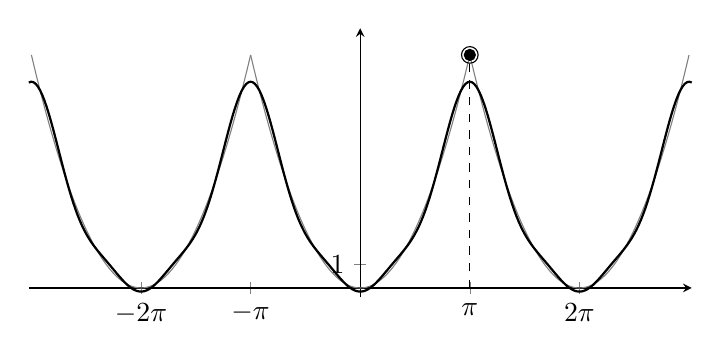
\begin{tikzpicture}
\begin{axis}[
    width=10cm, height=5cm,
    xmin=-9.5, xmax=9.5,
    ymin=-0.4, ymax=11,
    xtick={-6.2832,-3.1416,0,3.1416,6.2832},
    xticklabels={$-2\pi$,$-\pi$,$0$,$\pi$,$2\pi$},
    ytick={1},
    axis lines=center,
    samples=300,
    clip=false,
]
\addplot[thin, gray, domain=-3.1416:3.1416]    {x^2};
\addplot[thin, gray, domain=-9.4248:-3.1416]   {(x+6.2832)^2};
\addplot[thin, gray, domain=3.1416:9.4248]     {(x-6.2832)^2};
\addplot[thick, domain=-9.5:9.5]
    {9.8696/3 - 4*cos(deg(x)) + cos(deg(2*x)) - (4/9)*cos(deg(3*x))};
\draw[dashed] (axis cs:3.1416,0) -- (axis cs:3.1416,9.8696);
\addplot[only marks, mark=*, mark size=2pt] coordinates {(3.1416,9.8696)};
\addplot[only marks, mark=o,  mark size=3pt] coordinates {(3.1416,9.8696)};
\end{axis}
\end{tikzpicture}
\caption{Im Punkt $\pi$ haben wir Konvergenz gegen den Funktionswert $\pi^2$.
\label{basel:figure:konvergenz}}
\end{figure}

\subsection{Berechnung der Fourierpolynome}
\label{basel:subsection:berechnung}

Wir betrachten die Funktion
\[
    f(x) = x^2.
\]
Das allgemeine Fourierpolynom der Ordnung $n$ ist
\[
    F_n f(x)
    =
    \frac{a_0}{2}
    + \sum_{k=1}^{n} \bigl( a_k \cos(kx) + b_k \sin(kx) \bigr).
\]
Da $f(x) = x^2$ eine gerade Funktion ist, verschwinden alle Sinus-Koeffizienten:
\[
    b_k
    =
    \frac{1}{\pi} \int_{-\pi}^{\pi} x^2 \sin(kx)\, dx
    =
    0,
    \qquad (k > 0).
\]
Der Koeffizient $a_0$ ergibt sich zu
\[
    a_0
    =
    \frac{1}{\pi} \int_{-\pi}^{\pi} x^2\, dx
    =
    \frac{x^3}{3\pi} \Big|_{-\pi}^{\pi}
    =
    \frac{2\pi^2}{3}.
\]
Für $k > 0$ ergibt partielle Integration
\begin{align*}
    a_k
    &=
    \frac{1}{\pi} \int_{-\pi}^{\pi} x^2 \cos(kx)\, dx
    \\
    &=
    \frac{1}{k\pi}
    \left(
        x^2 \sin(kx) \Big|_{-\pi}^{\pi}
        - 2 \int_{-\pi}^{\pi} x \sin(kx)\, dx
    \right)
    \\
    &=
    -\frac{2}{k\pi} \int_{-\pi}^{\pi} x \sin(kx)\, dx
    \\
    &=
    \frac{2}{k^2\pi}
    \left(
        x \cos(kx) \Big|_{-\pi}^{\pi}
        - \int_{-\pi}^{\pi} \cos(kx)\, dx
    \right)
    \\
    &=
    \frac{2x}{k^2\pi} \cos(kx) \Big|_{-\pi}^{\pi}
    =
    (-1)^k \frac{4}{k^2},
    \qquad (k > 0).
\end{align*}
Damit ergibt sich die Fourierreihe von $f$:
\[
    f(x)
    =
    \frac{a_0}{2} + \sum_{k=1}^{\infty} \bigl( a_k \cos(kx) + b_k \sin(kx) \bigr)
    =
    \frac{\pi^2}{3} + 4 \sum_{k=1}^{\infty} \frac{(-1)^k}{k^2} \cos(kx).
\]
Nun wird $\pi^2 = f(\pi)$ eingesetzt:
\begin{equation}
    \pi^2
    =
    f(\pi)
    =
    \frac{\pi^2}{3}
    + 4 \sum_{k=1}^{\infty} \frac{(-1)^k}{k^2} \cos(k\pi)
    =
    \frac{\pi^2}{3} + \sum_{k=1}^{\infty} \frac{4}{k^2}.
    \label{basel:equation:einsetzung}
\end{equation}
